% Build with XeLaTeX or LuaLaTeX (Indic scripts).  Overleaf: Menu > Compiler > XeLaTeX.   Local: xelatex main && bibtex main && xelatex main && xelatex main
% Official ACL style files are in the same folder (acl.sty, acl_natbib.bst); they are unmodified copies of acl-org/acl-style-files.
\documentclass[11pt]{article}

% `preprint' = official ACL option that shows author names/affiliations (the demo track is single-blind) plus page numbers.
% Confirm against the OpenReview Demo Track instructions before submitting (see FINAL_CONTEXT.md, section "Venue checks").
\usepackage[preprint]{acl}
\usepackage{microtype}
\usepackage[english,bidi=default]{babel}
\babelfont{rm}{TeXGyreTermesX}            % Times-like main font, as in the official acl_lualatex.tex
\usepackage{fontspec}
% Noto Sans Devanagari / Gujarati are bundled in fonts/ (SIL OFL 1.1) so the build needs no system fonts.
\newfontfamily\hifont[Path=fonts/,Extension=.ttf,UprightFont=NotoSansDevanagari-Regular,BoldFont=NotoSansDevanagari-Bold,Script=Devanagari]{NotoSansDevanagari}
\newfontfamily\gufont[Path=fonts/,Extension=.ttf,UprightFont=NotoSansGujarati-Regular,BoldFont=NotoSansGujarati-Bold,Script=Gujarati]{NotoSansGujarati}
\newcommand{\hi}[1]{{\hifont #1}}   % Hindi and Marathi (Devanagari)
\newcommand{\gu}[1]{{\gufont #1}}   % Gujarati

\usepackage{booktabs,graphicx,amsmath,array,multirow,xcolor,enumitem,float}
\setlist{nosep,leftmargin=*}
% relax LaTeX's default float limits so tables stay near their text (does not alter the ACL style file)
\setcounter{topnumber}{3}\setcounter{bottomnumber}{2}\setcounter{totalnumber}{5}\setcounter{dbltopnumber}{3}
\renewcommand{\topfraction}{0.9}\renewcommand{\bottomfraction}{0.8}\renewcommand{\textfraction}{0.08}\renewcommand{\floatpagefraction}{0.75}\renewcommand{\dblfloatpagefraction}{0.75}
\newcolumntype{L}[1]{>{\raggedright\arraybackslash}p{#1}}
\newcommand{\sys}{\textsc{Indic AAC Studio}}
\newcommand{\nstated}{\textit{n.s.}}
\newcommand{\cn}[1]{\raisebox{.15ex}{\textcircled{\scriptsize #1}}}   % numbered callout
% AUTO-GENERATED by eval/make_tex.py from eval/results/*.json -- do not edit
\newcommand{\NScen}{184}
\newcommand{\NScenCM}{8}
\newcommand{\NOverlap}{9}
\newcommand{\NPrimEN}{46}
\newcommand{\NAllEN}{46}
\newcommand{\NPrimHI}{45}
\newcommand{\NAllHI}{46}
\newcommand{\NPrimGU}{42}
\newcommand{\NAllGU}{46}
\newcommand{\NPrimMR}{42}
\newcommand{\NAllMR}{46}
\newcommand{\NPrimAll}{175}
\newcommand{\PDNEN}{\mbox{+43\,pp [+28, +59]}}
\newcommand{\CDNEN}{22/46\,vs\,2/46}
\newcommand{\PDNHI}{\mbox{+67\,pp [+53, +80]}}
\newcommand{\CDNHI}{31/45\,vs\,1/45}
\newcommand{\PDNGU}{\mbox{+40\,pp [+24, +57]}}
\newcommand{\CDNGU}{21/42\,vs\,4/42}
\newcommand{\PDNMR}{\mbox{+52\,pp [+36, +69]}}
\newcommand{\CDNMR}{23/42\,vs\,1/42}
\newcommand{\PDTEN}{\mbox{\ensuremath{-}24\,pp [\ensuremath{-}37, \ensuremath{-}13]}}
\newcommand{\CDTEN}{22/46\,vs\,33/46}
\newcommand{\PDTHI}{\mbox{+0\,pp [+0, +0]}}
\newcommand{\CDTHI}{31/45\,vs\,31/45}
\newcommand{\PDTGU}{\mbox{\ensuremath{-}14\,pp [\ensuremath{-}26, \ensuremath{-}5]}}
\newcommand{\CDTGU}{21/42\,vs\,27/42}
\newcommand{\PDTMR}{\mbox{\ensuremath{-}10\,pp [\ensuremath{-}21, +0]}}
\newcommand{\CDTMR}{23/42\,vs\,27/42}
\newcommand{\PDPEN}{\mbox{+41\,pp [+26, +57]}}
\newcommand{\CDPEN}{22/46\,vs\,3/46}
\newcommand{\PDPHI}{\mbox{+16\,pp [+7, +27]}}
\newcommand{\CDPHI}{31/45\,vs\,24/45}
\newcommand{\PDPGU}{\mbox{+2\,pp [+0, +7]}}
\newcommand{\CDPGU}{21/42\,vs\,20/42}
\newcommand{\PDPMR}{\mbox{+12\,pp [+2, +24]}}
\newcommand{\CDPMR}{23/42\,vs\,18/42}
\newcommand{\PSUEN}{\mbox{+24\,pp [+13, +37]}}
\newcommand{\CSUEN}{33/46\,vs\,22/46}
\newcommand{\PSUHI}{\mbox{+22\,pp [+11, +36]}}
\newcommand{\CSUHI}{41/45\,vs\,31/45}
\newcommand{\PSUGU}{\mbox{+12\,pp [+2, +21]}}
\newcommand{\CSUGU}{26/42\,vs\,21/42}
\newcommand{\PSUMR}{\mbox{+21\,pp [+7, +36]}}
\newcommand{\CSUMR}{32/42\,vs\,23/42}
\newcommand{\PSTEN}{\mbox{\ensuremath{-}28\,pp [\ensuremath{-}41, \ensuremath{-}15]}}
\newcommand{\CSTEN}{33/46\,vs\,46/46}
\newcommand{\PSTHI}{\mbox{\ensuremath{-}9\,pp [\ensuremath{-}18, \ensuremath{-}2]}}
\newcommand{\CSTHI}{41/45\,vs\,45/45}
\newcommand{\PSTGU}{\mbox{\ensuremath{-}19\,pp [\ensuremath{-}31, \ensuremath{-}7]}}
\newcommand{\CSTGU}{26/42\,vs\,34/42}
\newcommand{\PSTMR}{\mbox{\ensuremath{-}24\,pp [\ensuremath{-}38, \ensuremath{-}12]}}
\newcommand{\CSTMR}{32/42\,vs\,42/42}
\newcommand{\PSPEN}{\mbox{+61\,pp [+46, +74]}}
\newcommand{\CSPEN}{33/46\,vs\,5/46}
\newcommand{\PSPHI}{\mbox{+33\,pp [+20, +47]}}
\newcommand{\CSPHI}{41/45\,vs\,26/45}
\newcommand{\PSPGU}{\mbox{+24\,pp [+12, +38]}}
\newcommand{\CSPGU}{26/42\,vs\,16/42}
\newcommand{\PSPMR}{\mbox{+19\,pp [+7, +31]}}
\newcommand{\CSPMR}{32/42\,vs\,24/42}
\newcommand{\PLLEN}{\mbox{\ensuremath{-}4\,pp [\ensuremath{-}11, +0]}}
\newcommand{\CLLEN}{1/46\,vs\,3/46}
\newcommand{\PLLHI}{\mbox{+0\,pp [+0, +0]}}
\newcommand{\CLLHI}{24/45\,vs\,24/45}
\newcommand{\PLLGU}{\mbox{+0\,pp [+0, +0]}}
\newcommand{\CLLGU}{20/42\,vs\,20/42}
\newcommand{\PLLMR}{\mbox{+0\,pp [+0, +0]}}
\newcommand{\CLLMR}{18/42\,vs\,18/42}
\newcommand{\FBUAll}{61/184}
\newcommand{\FBUEN}{30/46}
\newcommand{\FBpctUEN}{65\%}
\newcommand{\ErrUEN}{0}
\newcommand{\FBUHI}{8/46}
\newcommand{\FBpctUHI}{17\%}
\newcommand{\ErrUHI}{0}
\newcommand{\FBUGU}{6/46}
\newcommand{\FBpctUGU}{13\%}
\newcommand{\ErrUGU}{0}
\newcommand{\FBUMR}{17/46}
\newcommand{\FBpctUMR}{37\%}
\newcommand{\ErrUMR}{0}
\newcommand{\FBSAll}{67/184}
\newcommand{\FBSEN}{28/46}
\newcommand{\FBpctSEN}{61\%}
\newcommand{\ErrSEN}{0}
\newcommand{\FBSHI}{15/46}
\newcommand{\FBpctSHI}{33\%}
\newcommand{\ErrSHI}{0}
\newcommand{\FBSGU}{16/46}
\newcommand{\FBpctSGU}{35\%}
\newcommand{\ErrSGU}{0}
\newcommand{\FBSMR}{8/46}
\newcommand{\FBpctSMR}{17\%}
\newcommand{\ErrSMR}{0}
\newcommand{\LatAllEN}{11.75\,s (p90 12.75, n=69)}
\newcommand{\LatAcceptedEN}{6.05\,s (p90 6.23, n=22)}
\newcommand{\LatFallbackEN}{12.04\,s (p90 12.81, n=47)}
\newcommand{\LatAllHI}{9.97\,s (p90 18.85, n=70)}
\newcommand{\LatAcceptedHI}{9.75\,s (p90 10.08, n=52)}
\newcommand{\LatFallbackHI}{18.76\,s (p90 20.12, n=18)}
\newcommand{\LatAllGU}{7.5\,s (p90 14.77, n=72)}
\newcommand{\LatAcceptedGU}{7.45\,s (p90 7.58, n=51)}
\newcommand{\LatFallbackGU}{14.73\,s (p90 15.06, n=21)}
\newcommand{\LatAllMR}{6.58\,s (p90 13.05, n=72)}
\newcommand{\LatAcceptedMR}{6.51\,s (p90 7.06, n=49)}
\newcommand{\LatFallbackMR}{13.0\,s (p90 13.81, n=23)}
\newcommand{\LatMedAccEN}{6.05}
\newcommand{\LatMedFbEN}{12.04}
\newcommand{\LatMedAccHI}{9.75}
\newcommand{\LatMedFbHI}{18.76}
\newcommand{\LatMedAccGU}{7.45}
\newcommand{\LatMedFbGU}{14.73}
\newcommand{\LatMedAccMR}{6.51}
\newcommand{\LatMedFbMR}{13.0}
\newcommand{\LatFbMin}{12.04}
\newcommand{\LatFbMax}{18.76}
\newcommand{\NUniqueReq}{283}
\newcommand{\StageLlmOne}{1.87}
\newcommand{\StageLlmTwo}{0.0}
\newcommand{\StageLlmThree}{4.63}
\newcommand{\StageSem}{0.0}
\newcommand{\StageTts}{0.0}
\newcommand{\StageTotal}{9.46}
\newcommand{\PredENOneInf}{17.2}
\newcommand{\PredENOneTri}{16.0}
\newcommand{\PredENFiveInf}{33.4}
\newcommand{\PredENFiveTri}{32.8}
\newcommand{\PredDENOneTri}{\mbox{+1.1\,pp [+0.5, +1.8]}}
\newcommand{\PredDENFiveTri}{\mbox{+0.6\,pp [+0.0, +1.2]}}
\newcommand{\PredDENMrrTri}{\mbox{+0.007 [+0.002, +0.011]}}
\newcommand{\PredDENOneBi}{\mbox{+3.6\,pp [+2.3, +5.0]}}
\newcommand{\PredDENFiveBi}{\mbox{+3.9\,pp [+2.7, +5.1]}}
\newcommand{\PredDENMrrBi}{\mbox{+0.036 [+0.025, +0.049]}}
\newcommand{\PredDENOneUni}{\mbox{+13.5\,pp [+11.4, +15.7]}}
\newcommand{\PredDENFiveUni}{\mbox{+21.8\,pp [+19.0, +24.8]}}
\newcommand{\PredDENMrrUni}{\mbox{+0.171 [+0.148, +0.197]}}
\newcommand{\PredNEN}{2220}
\newcommand{\PredClustersEN}{60}
\newcommand{\PredOOVEN}{7.5\%}
\newcommand{\PredHIOneInf}{27.0}
\newcommand{\PredHIOneTri}{25.9}
\newcommand{\PredHIFiveInf}{44.1}
\newcommand{\PredHIFiveTri}{44.0}
\newcommand{\PredDHIOneTri}{\mbox{+1.2\,pp [+0.5, +1.9]}}
\newcommand{\PredDHIFiveTri}{\mbox{+0.1\,pp [\ensuremath{-}0.3, +0.4]}}
\newcommand{\PredDHIMrrTri}{\mbox{+0.008 [+0.004, +0.013]}}
\newcommand{\PredDHIOneBi}{\mbox{+3.0\,pp [+1.8, +4.3]}}
\newcommand{\PredDHIFiveBi}{\mbox{+1.0\,pp [+0.1, +1.9]}}
\newcommand{\PredDHIMrrBi}{\mbox{+0.023 [+0.014, +0.032]}}
\newcommand{\PredDHIOneUni}{\mbox{+20.6\,pp [+18.4, +23.0]}}
\newcommand{\PredDHIFiveUni}{\mbox{+29.5\,pp [+26.8, +32.4]}}
\newcommand{\PredDHIMrrUni}{\mbox{+0.243 [+0.220, +0.267]}}
\newcommand{\PredNHI}{2437}
\newcommand{\PredClustersHI}{60}
\newcommand{\PredOOVHI}{5.5\%}
\newcommand{\UIFalseNeg}{3}
\newcommand{\UISingle}{276}
\newcommand{\UIFeelReq}{27}
\newcommand{\GateAccU}{116}
\newcommand{\GateAccOkU}{57}
\newcommand{\GateAccPctU}{49\%}
\newcommand{\GateFbU}{59}
\newcommand{\GateFbOkU}{40}
\newcommand{\GateFbPctU}{68\%}
\newcommand{\GateAccS}{108}
\newcommand{\GateAccOkS}{71}
\newcommand{\GateAccPctS}{66\%}
\newcommand{\GateFbS}{67}
\newcommand{\GateFbOkS}{61}
\newcommand{\GateFbPctS}{91\%}
\newcommand{\CMSuccNaive}{0/8}
\newcommand{\CMSuccPre}{0/8}
\newcommand{\CMSuccDepU}{4/8}
\newcommand{\CMSuccDepS}{5/8}
\newcommand{\CMSuccTmplU}{6/8}
\newcommand{\CMSuccTmplS}{8/8}
\newcommand{\ActWrongUEN}{12/46}
\newcommand{\SuccEffUEN}{22/46}
\newcommand{\ActWrongSEN}{2/46}
\newcommand{\SuccEffSEN}{33/46}
\newcommand{\ActWrongUHI}{14/45}
\newcommand{\SuccEffUHI}{31/45}
\newcommand{\ActWrongSHI}{4/45}
\newcommand{\SuccEffSHI}{41/45}
\newcommand{\ActWrongUGU}{11/42}
\newcommand{\SuccEffUGU}{21/42}
\newcommand{\ActWrongSGU}{2/42}
\newcommand{\SuccEffSGU}{26/42}
\newcommand{\ActWrongUMR}{17/42}
\newcommand{\SuccEffUMR}{23/42}
\newcommand{\ActWrongSMR}{9/42}
\newcommand{\SuccEffSMR}{32/42}
\newcommand{\GutHitOne}{6.7}
\newcommand{\HiHmmHitOne}{24.5}
\newcommand{\CPzeroPol}{2.1\%}
\newcommand{\CPallConcept}{98.3\%}
\newcommand{\SuccNaive}{8/175}
\newcommand{\SuccPctNaive}{5\%}
\newcommand{\KeptNaive}{199/215}
\newcommand{\KeptPctNaive}{93\%}
\newcommand{\PolErrNaive}{2/175}
\newcommand{\ActWrongNaive}{3/175}
\newcommand{\AddedNaive}{7/175}
\newcommand{\OffNaive}{16/175}
\newcommand{\SuccPre}{65/175}
\newcommand{\SuccPctPre}{37\%}
\newcommand{\KeptPre}{175/215}
\newcommand{\KeptPctPre}{81\%}
\newcommand{\PolErrPre}{2/175}
\newcommand{\ActWrongPre}{54/175}
\newcommand{\AddedPre}{25/175}
\newcommand{\OffPre}{19/175}
\newcommand{\SuccDepU}{97/175}
\newcommand{\SuccPctDepU}{55\%}
\newcommand{\KeptDepU}{215/215}
\newcommand{\KeptPctDepU}{100\%}
\newcommand{\PolErrDepU}{0/175}
\newcommand{\ActWrongDepU}{54/175}
\newcommand{\AddedDepU}{4/175}
\newcommand{\OffDepU}{10/175}
\newcommand{\SuccDepS}{132/175}
\newcommand{\SuccPctDepS}{75\%}
\newcommand{\KeptDepS}{215/215}
\newcommand{\KeptPctDepS}{100\%}
\newcommand{\PolErrDepS}{0/175}
\newcommand{\ActWrongDepS}{17/175}
\newcommand{\AddedDepS}{3/175}
\newcommand{\OffDepS}{9/175}
\newcommand{\SuccTmplS}{167/175}
\newcommand{\SuccPctTmplS}{95\%}
\newcommand{\KeptTmplS}{215/215}
\newcommand{\KeptPctTmplS}{100\%}
\newcommand{\PolErrTmplS}{0/175}
\newcommand{\ActWrongTmplS}{0/175}
\newcommand{\AddedTmplS}{0/175}
\newcommand{\OffTmplS}{0/175}
\newcommand{\SuccTmplU}{118/175}
\newcommand{\SuccPctTmplU}{67\%}
\newcommand{\KeptTmplU}{215/215}
\newcommand{\KeptPctTmplU}{100\%}
\newcommand{\PolErrTmplU}{0/175}
\newcommand{\ActWrongTmplU}{57/175}
\newcommand{\AddedTmplU}{0/175}
\newcommand{\OffTmplU}{0/175}
\newcommand{\SuccLit}{0/175}
\newcommand{\SuccPctLit}{0\%}
\newcommand{\KeptLit}{215/215}
\newcommand{\KeptPctLit}{100\%}
\newcommand{\PolErrLit}{0/175}
\newcommand{\ActWrongLit}{0/175}
\newcommand{\AddedLit}{0/175}
\newcommand{\OffLit}{0/175}
\newcommand{\RefARules}{384/384}
\newcommand{\RefARulesPct}{100.0\%}
\newcommand{\RefAModel}{378/384}
\newcommand{\RefAModelPct}{98.4\%}
\newcommand{\RefAHybrid}{384/384}
\newcommand{\RefAHybridPct}{100.0\%}
\newcommand{\RefARaw}{0/384}
\newcommand{\RefARawPct}{0.0\%}
\newcommand{\RefALat}{31.8}
\newcommand{\RefFRules}{384/384}
\newcommand{\RefFRulesPct}{100.0\%}
\newcommand{\RefFModel}{379/384}
\newcommand{\RefFModelPct}{98.7\%}
\newcommand{\RefFHybrid}{384/384}
\newcommand{\RefFHybridPct}{100.0\%}
\newcommand{\RefFRaw}{0/384}
\newcommand{\RefFRawPct}{0.0\%}
\newcommand{\RefFLat}{32.2}
\newcommand{\IGSent}{15{,}505}
\newcommand{\IGTok}{112{,}875}
\newcommand{\IGDepth}{181}
\newcommand{\OffReady}{10.2}
\newcommand{\OffFirstEn}{13.94}
\newcommand{\OffHi}{10.1}
\newcommand{\NSymbols}{69}
\newcommand{\NCategories}{9}
   % every number below is regenerated from eval/results by eval/make_tex.py

\title{Concept-Gated Symbol-to-Speech Generation for English, Hindi, Gujarati and Marathi AAC}

% Single-blind: names and affiliations are shown. PLACEHOLDER: no authoritative author list exists in the project records.
\author{\textbf{{[Author names]}} \\
  {[Affiliations]} \\
  \texttt{{[contact e-mail]}}}

\begin{document}
\maketitle

\begin{abstract}
Users of symbol-based augmentative and alternative communication (AAC) produce telegraphic selections that a language model can expand into sentences, but the expansion may drop a selected concept, invert polarity, or add content the user did not choose.
We present \sys{}, a web system for English, Hindi, Gujarati and Marathi that expands symbol selections with a prompted Qwen2.5-0.5B cascade, accepts the output only if a deterministic validator confirms the selected concepts, polarity and intent, and otherwise returns a template built from the user's own labels.
Trained next-word predictors and zero-shot IndicF5 speech complete the system.
On \NPrimAll{} frozen, paired scenarios in four languages, the gate raises the cascade's concept retention from \KeptPctPre{} to \KeptPctDepU{} and its scenario-level success from \SuccPctPre{} to \SuccPctDepU{}, against \SuccPctNaive{} for an unconstrained prompt; explicit polarity and intent fields raise success to \SuccPctDepS{}.
A template-only baseline reaches \SuccPctTmplS{} under those fields, and a failure analysis identifies the defects that limit the cascade.
The system, fixtures and scorer accompany the submission.
\end{abstract}

\section{Introduction}
\label{sec:intro}

A person who communicates through an AAC board composes a message by selecting symbols, and a speech-generating device voices the selected labels.
The result is telegraphic: \emph{Water}, or \emph{No}+\emph{Pizza}. A language model can expand such selections into sentences, and Indian-language boards would benefit from this because Hindi, Gujarati and Marathi require agreement, postpositions and negation forms that a literal join of labels cannot supply.
For AAC, however, fluency is not sufficient, because the device speaks on behalf of the user and the listener cannot see the selection.
Three outputs of the cascade evaluated in this paper illustrate the risk: for \emph{Water} it produced ``I need food.'' (a concept replaced); for \emph{No}+\emph{Water} in Marathi it produced \hi{मला पाणी हवे आहे.} (``I want water''; polarity inverted); and for \emph{Tired} it produced ``The user is tired of waiting for their meal and wants to go out to eat.'' (content added).

\sys{} addresses this with a \emph{concept gate}. The selection is converted into a ledger of required and forbidden concepts, a prompted cascade realizes a sentence, a deterministic validator accepts it only if the ledger is satisfied, and a template built from the user's own labels replaces it otherwise.
The system adds a four-locale symbol board, trained next-word predictors and zero-shot voice synthesis. We contribute:
\begin{itemize}
\item the gated realization pipeline and its acceptance rule (\S\ref{sec:system}), with an API that carries polarity and intent explicitly;
\item a frozen, paired evaluation with baselines, an independent scorer and a failure analysis (\S\ref{sec:eval}), and the fixtures and scorer for reuse;
\item trained English and Hindi predictors, evaluated on held-out conversations, and the end-to-end system with its demonstration walkthrough (Figures~\ref{fig:arch} and~\ref{fig:ui}).
\end{itemize}

\section{Related Work}
\label{sec:related}

\paragraph{Generative AAC from text or speech.}
ConnecTone \citep{francis2024connectone} suggests text from conversation context captured by speech recognition and voices it with a TTS that moves between reading and conversational style; its abstract reports no evaluation.
\citet{mohan2024composition} add LLM phrase suggestions with an emotional tone to typed, emoji or spoken input and voice the result in the user's own voice.
SpeakFaster \citep{cai2024speakfaster} expands abbreviated text for eye-gaze typing; it reports 57\% more saved motor actions than predictive keyboards in simulation and text-entry rates 29--60\% above baselines for two users with ALS.
All three start from letters or speech. \sys{} starts from symbol selections, which give the model a small concept set whose omission or inversion is checkable.

\paragraph{Symbols, voices and boards.}
\citet{francis2025static} generate symbols with DALL-E~3 and clone voices with XTTS on a Proloquo2Go-like board, but describe no sentence realization and report no evaluation; we adopt their interaction pattern.
The symbol boards Cboard, Jellow and Avaz \citep{cboard,jellow,avaz} state 46, an unspecified number and ``15+'' languages, do not name Hindi, Gujarati or Marathi for their apps (Jellow offers a Hindi website), and do not mention LLM sentence generation.
\citet{vertanen2026multilingual} releases AAC text in 34 languages; its table lists no Hindi, Gujarati or Marathi.

\paragraph{Gap.}
Table~\ref{tab:related} compares documented capabilities (\nstated{}: not stated by the source, not absent); external results are not comparable to ours.
Among these sources, none documents a deterministic concept-and-polarity gate over LLM output on a symbol board for an Indian language; we make no claim about undocumented products.
We therefore test the gate against matched baselines on one protocol (\S\ref{sec:eval}).

\begin{table*}[t]
\centering\footnotesize
\setlength{\tabcolsep}{3pt}
\begin{tabular}{@{}L{2.0cm}L{2.2cm}L{2.3cm}L{2.3cm}L{2.0cm}L{1.8cm}L{1.7cm}@{}}
\toprule
System & Input & Languages & LLM realization & Polarity / intent & Speech & Evaluation \\
\midrule
ConnecTone & partner speech, text & \nstated & text suggestions from context & \nstated & style-adaptive TTS & none in abstract \\
\citet{francis2025static} & symbols (generated images) & \nstated & none described & --- & zero-shot cloning & none reported \\
\citet{mohan2024composition} & typed, emoji, spoken & \nstated & phrase suggestions & \nstated & user's own voice & \nstated \\
SpeakFaster & abbreviated text (gaze) & \nstated & abbreviation expansion & --- & \nstated & simulation; 19 + 2 users \\
Cboard, Jellow, Avaz & symbols, icons, text & 46; Hindi site; 15+ (HI, GU, MR not stated for apps) & \nstated & \nstated & TTS (Cboard, Jellow) & \nstated \\
\midrule
\sys{} (ours) & symbols, text & EN, HI, GU, MR; Hinglish flag & prompted Qwen cascade & explicit fields; concept and polarity gate & IndicF5 + Vocos & this paper \\
\bottomrule
\end{tabular}
\caption{Documented capabilities of the closest systems, from the cited paper or the vendor page read on 2026-11-11. \nstated{}: not stated.}
\label{tab:related}
\end{table*}

\section{System Design and Demo Walkthrough}
\label{sec:system}

\begin{figure*}[t]
\centering
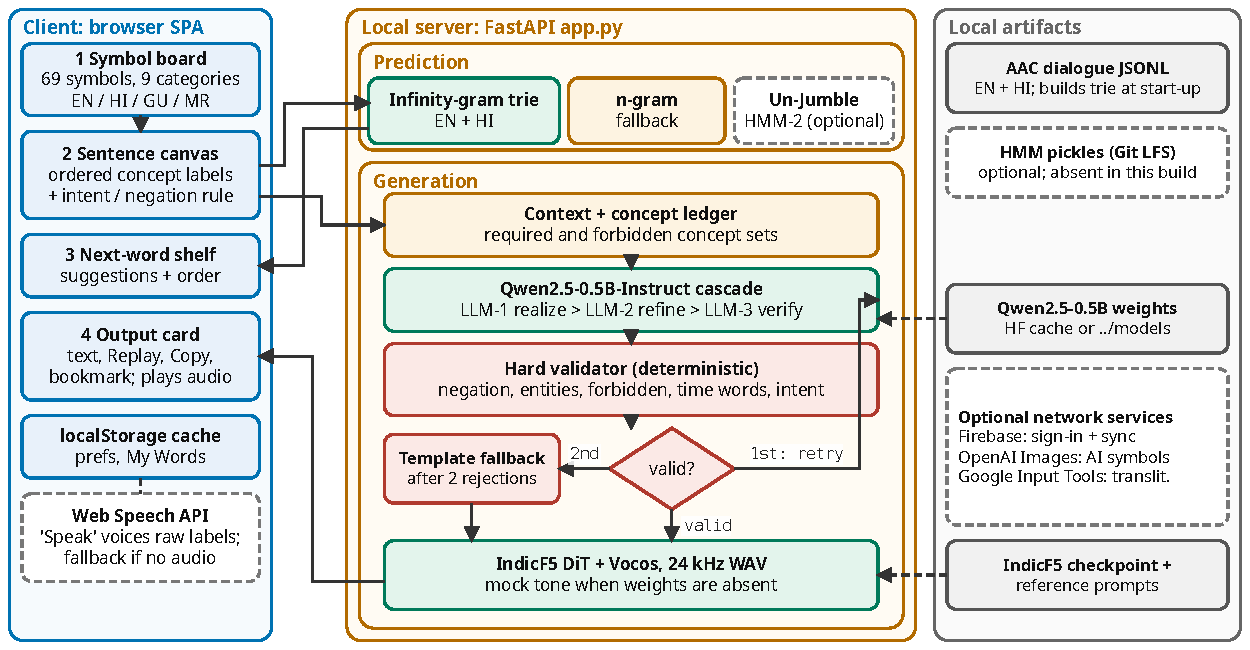
\includegraphics[width=\textwidth]{figures/architecture.pdf}
\caption{Architecture of the evaluated build. Solid boxes run locally; dashed boxes are optional or were absent (Git LFS HMM checkpoints, IndicF5 weights, network services). Between the columns, words flow to \texttt{/predict\_next}, the concept request to \texttt{/generate}, and text with \texttt{audio\_b64} back to the output card.}
\label{fig:arch}
\end{figure*}

\paragraph{Walkthrough.}
The user selects a language and taps symbols from a board of \NSymbols{} symbols in \NCategories{} categories, labeled in English, Hindi, Gujarati and Marathi (Figure~\ref{fig:ui}, \cn{1}); free text, an emoji search and a per-user ``My Words'' grid extend the vocabulary.
Selections accumulate on a sentence canvas (\cn{2}) while a shelf proposes next words (\cn{3}).
\emph{Speak} voices the literal labels with the browser's speech synthesis; \emph{AI Polish \& Speak} (\cn{4}) sends the selection to the local server and shows the returned sentence on an output card (\cn{5}) with Replay, Copy and bookmark controls.
The card is for review; the user revises a sentence by editing the canvas and regenerating.

\begin{figure*}[t]
\centering
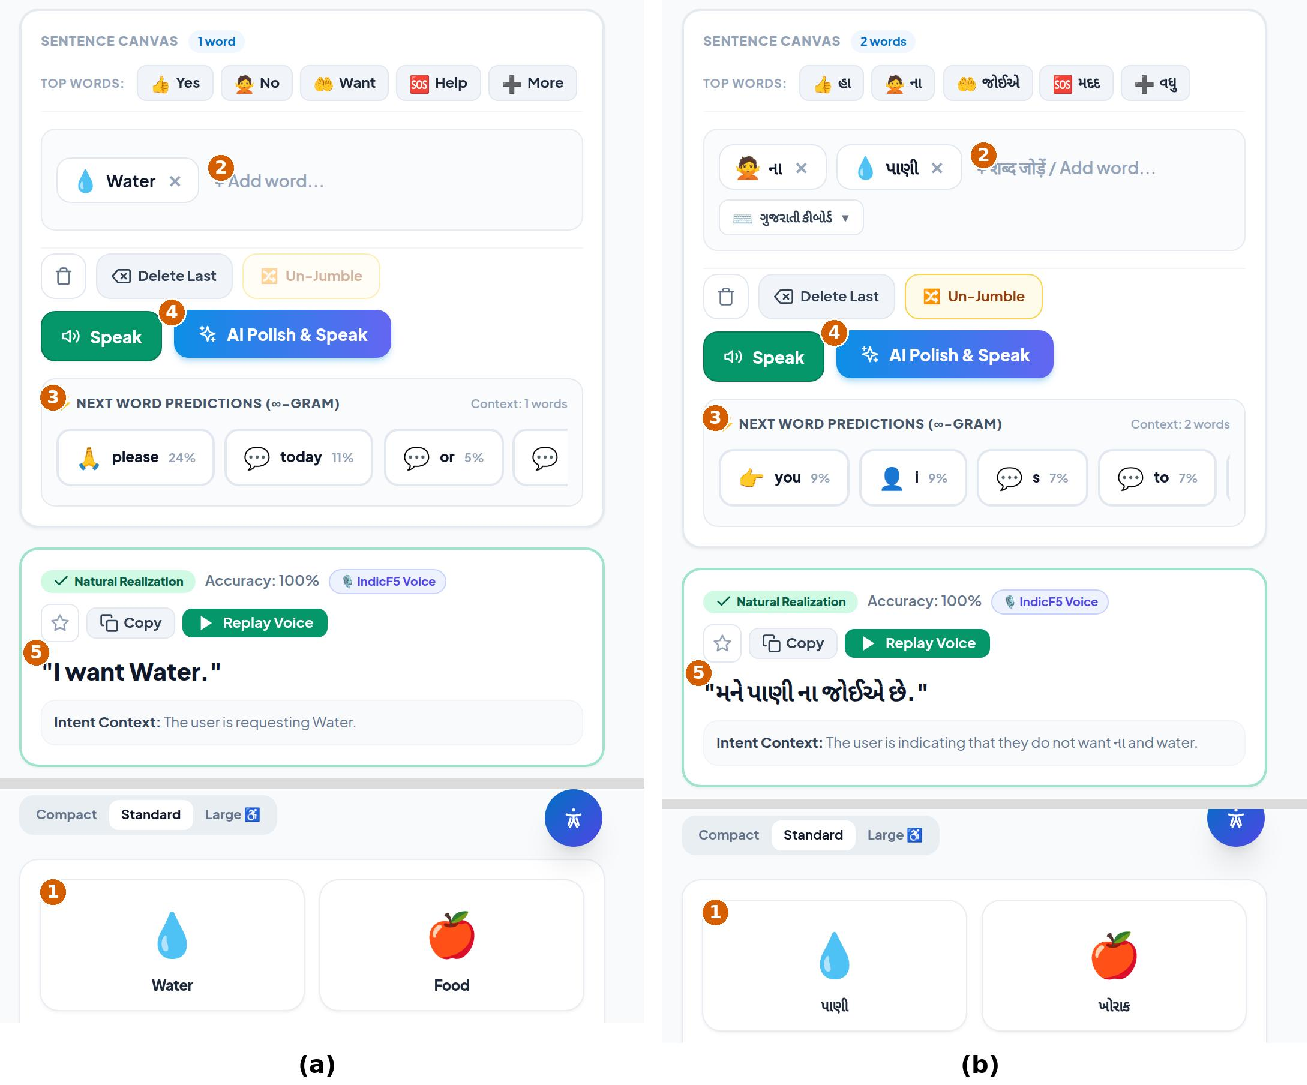
\includegraphics[width=0.74\textwidth]{figures/ui_panel.pdf}
\caption{Screenshots of the running build (Chrome, 520\,px viewport, signed-out default profile). (a)~English, \emph{Water}: the cascade output was rejected and the template returned. (b)~Gujarati, \gu{ના}+\gu{પાણી} (``no''+``water''): the cascade output was accepted; the shelf suggests English words (\S\ref{sec:eval}). Callouts: \cn{1} selected symbol, \cn{2} canvas, \cn{3} next-word shelf, \cn{4} generate, \cn{5} output sentence.}
\label{fig:ui}
\end{figure*}

\paragraph{Request and concept ledger.}
The client posts the ordered labels as \texttt{entities}, with \texttt{intent}, \texttt{negation}, \texttt{language}, \texttt{code\_mix}, \texttt{generation\_mode} and \texttt{voice\_id}, to \texttt{/generate}.
The web client infers \texttt{intent} and \texttt{negation} by substring rules over the labels (\textsc{negation} if a label contains \emph{no}, \emph{not} or a Hindi, Gujarati or Marathi negator; \textsc{question} for question words; \textsc{statement} for happy, sad, love and two Hindi labels; otherwise \textsc{request}); the API accepts the same fields from any client.
The server builds a \emph{ledger}: a required set (intent, actor, each selected entity, negation) and a forbidden set of 21 default words for unrequested times, meals and venues (e.g., \emph{tomorrow}, \emph{restaurant}), minus any word the user selected.

\paragraph{Realization and validation.}
Three prompted stages share one frozen Qwen2.5-0.5B-Instruct \citep{qwen2025qwen25}. LLM-1 realizes a sentence, from a few-shot prompt for Hindi, Gujarati and Marathi (12, 9 and 9 examples; greedy decoding) and from a ledger prompt for English and code-mixed output (temperature 0.1); LLM-2 removes unsupported content and is skipped for Indic-script candidates; LLM-3 returns a JSON verdict and a minimal rewrite.
A deterministic validator then decides. With $\nu$ the negation flag, $E$ the selected entities, $F$ the forbidden set and $y$ the candidate,
\begin{multline}
\mathrm{accept}(y)=[\mathrm{neg}(y)=\nu]\wedge\mathrm{match}(E,y)\\
\wedge\mathrm{intent}(y)\wedge\neg\mathrm{forbid}_F(y)\wedge\neg\mathrm{time}(y).
\label{eq:gate}
\end{multline}
Here \emph{neg} tests a fixed list of English, Hindi, Gujarati and Marathi negators; \emph{match} requires every selected entity to appear (a substring, plural and Indic-stem test); \emph{intent} rejects ``I want'' for feeling intents and requires a question cue for questions; \emph{forbid} matches words of $F$; and \emph{time} flags time words when none was selected.
A score in $[0,1]$ is displayed as \emph{Accuracy}, but the gate has no numeric threshold.
A rejection triggers one more cascade run; after two rejections a language-specific template built from the selected labels is returned (e.g., ``I want Water.'').
English and code-mixed attempts differ because LLM-1 samples; Indic attempts repeat because decoding is greedy.
The template is returned even if it fails the validator, and the card does not show that a fallback occurred.

\paragraph{Prediction and speech.}
Next-word suggestions come from an unbounded-order suffix-trie model with backoff 0.4, in the spirit of infini-gram \citep{liu2024infinigram}, built at start-up from the English and Hindi dialogue files (\IGSent{} sentences, \IGTok{} tokens); the trained HMMs serve as fallback and for \emph{Un-Jumble}.
Accepted text is synthesized by IndicF5 \citep{ai4bharat2025indicf5}, a flow-matching model of the F5-TTS family \citep{chen2025f5tts}, with a 24\,kHz Vocos vocoder \citep{siuzdak2023vocos}; a reference clip and its transcript condition the voice zero-shot.

\paragraph{Models and training.}
Table~\ref{tab:models} lists the learned components. The LLM and the speech model are used as released.
HMM-1 (interpolated 4-gram) and HMM-2 (word-and-POS trigram decoder) are trained by streaming external English text; the Hindi HMM and the infinity-gram model are trained on the AAC dialogues; an English flan-T5-small refiner is fine-tuned on template-generated payloads and reproduces at \RefAModelPct{} exact match on 384 group-disjoint payloads (Appendix~\ref{app:refiner}), but the server does not load it.

\begin{table*}[t]
\centering\footnotesize
\setlength{\tabcolsep}{3pt}
\begin{tabular}{@{}L{2.6cm}L{2.1cm}L{6.2cm}L{2.0cm}L{1.7cm}@{}}
\toprule
Component & Role & Training or adaptation & Data & In demo path \\
\midrule
Qwen2.5-0.5B-Instruct (rev.\ 7ae5576) & LLM-1/2/3 & None; prompted (few-shot for HI, GU, MR) & -- & yes \\
IndicF5 + Vocos & speech & Pretrained; zero-shot voice conditioning on a clip and transcript & 1,417\,h (4 corpora) & yes; weights not bundled \\
HMM-1, HMM-2 & next word; un-jumble & Streaming, 500K-sentence chunks (3 high-quality English, 2 Tatoeba, up to 500 Pile; log outside the artifact); pruning at counts 3 and 2. HMM-1: Jelinek--Mercer .50/.30/.15/.05. HMM-2: word and POS trigrams; exact search to 6 words, beam 64 above & external English text & yes, if checkpoints present \\
Gutenberg HMM & English bigram, trigram & 188,402 sentences; 63,783 bigram and 713,845 trigram states & public-domain books & legacy; Table~\ref{tab:pred} \\
Hindi AAC HMM & Hindi fallback & 3,867 turns of the Hindi dialogues; 2,171 word types & Hindi dialogues & fallback \\
Infinity-gram & next word (primary) & Count-based suffix trie built at start-up & EN, HI dialogues & yes \\
flan-T5-small refiner & English realization & Fine-tuned: 10 epochs (960 updates), learning rate $10^{-4}$, effective batch 32, seed 42 (Appendix~\ref{app:refiner}) & 3,052 template payloads & no \\
\bottomrule
\end{tabular}
\caption{Learned components. Sources: training scripts, run configurations and pickles in the artifact; the HMM-1 and HMM-2 checkpoints are Git LFS objects that were not available during evaluation. The four IndicF5 corpora are Rasa, IndicTTS, LIMMITS and IndicVoices-R.}
\label{tab:models}
\end{table*}

\section{Evaluation}
\label{sec:eval}

\paragraph{Protocol.}
We froze \NScen{} scenarios before scoring any output: per language (English, Hindi, Gujarati, Marathi) 46 selections from the board vocabulary, namely a food request (10), a refusal (\emph{No}+food; 10), a feeling (8), a negated feeling (8), an action and object (6), and \emph{Help} or \emph{Call} with a person (4), with gold polarity and act fixed by the grid; eight Hinglish scenarios form an exploratory block.
Each scenario is sent as the web client builds it (\emph{client}) and with explicit \texttt{intent} and \texttt{negation} fields (\emph{structured}). We compare a literal join of the labels; the backend template alone; the same Qwen model with one unconstrained prompt (no ledger, examples, verifier or gate); the cascade output before the gate, taken from the same response as the deployed output so that gate and fallback are isolated on identical candidates; and the deployed output of the live \texttt{/generate} endpoint.
A scenario \emph{succeeds} if the output keeps every selected concept, has the gold polarity and act, adds no unselected concept, and is a first-person sentence in the target script.
A lexical scorer written independently of the validator applies these rules (Appendix~\ref{app:scorer}); its Indic lexicon is not native-reviewed.
Nine scenarios whose few-shot prompt reproduces a prompt example are excluded, leaving \NPrimAll{} (\NPrimEN{}, \NPrimHI{}, \NPrimGU{}, \NPrimMR{}).
Differences are paired by scenario with 95\% bootstrap intervals (10,000 resamples). Runs used one GTX 1650 (4\,GB); English and code-mixed outputs are single samples because LLM-1 samples.

\begin{table*}[t]\centering\footnotesize\setlength{\tabcolsep}{2.6pt}
\begin{tabular}{@{}p{3.5cm}ccccc@{\hspace{8pt}}ccccc@{}}
\toprule
 & \multicolumn{5}{c}{Scenario success (n/N)} & \multicolumn{5}{c}{Pooled error decomposition (lower is better)} \\
\cmidrule(lr){2-6}\cmidrule(lr){7-11}
System & EN & HI & GU & MR & All & Kept & Polarity & Act & Added & Off-task \\
\midrule
Literal join & 0/46 & 0/45 & 0/42 & 0/42 & 0/175 & 215/215 & 0/175 & 0/175 & 0/175 & 0/175 \\
Template only (client) & 33/46 & 31/45 & 27/42 & 27/42 & 118/175 & 215/215 & 0/175 & 57/175 & 0/175 & 0/175 \\
Prompted Qwen, no gate & 2/46 & 1/45 & 4/42 & 1/42 & 8/175 & 199/215 & 2/175 & 3/175 & 7/175 & 16/175 \\
Cascade before gate (client) & 3/46 & 24/45 & 20/42 & 18/42 & 65/175 & 175/215 & 2/175 & 54/175 & 25/175 & 19/175 \\
\textbf{Deployed (client)} & 22/46 & 31/45 & 21/42 & 23/42 & 97/175 & 215/215 & 0/175 & 54/175 & 4/175 & 10/175 \\
\midrule
Template only (struct.) & 46/46 & 45/45 & 34/42 & 42/42 & 167/175 & 215/215 & 0/175 & 0/175 & 0/175 & 0/175 \\
\textbf{Deployed (struct.)} & 33/46 & 41/45 & 26/42 & 32/42 & 132/175 & 215/215 & 0/175 & 17/175 & 3/175 & 9/175 \\
\bottomrule
\end{tabular}
\caption{Primary set (175 scenarios; EN 46, HI 45, GU 42, MR 42). Left: scenarios whose output keeps every selected concept, has the gold polarity and act, adds no unselected concept and is an on-task first-person sentence (independent lexical scorer). Right (pooled): required concept instances kept (of 215) and scenarios with a wrong polarity, wrong act, added concept or off-task output. Client = payload built by the web client; struct. = explicit intent and negation fields.}
\label{tab:results}
\end{table*}


\paragraph{Results.}
Table~\ref{tab:results} reports the primary set.
Before the gate, the cascade keeps \KeptPctPre{} of required concepts and succeeds on \SuccPctPre{} of scenarios; with gate and fallback the same requests keep \KeptDepU{} (\KeptPctDepU{}; 95\% lower bound \CPallConcept{}) and succeed on \SuccPctDepU{}, a paired gain of \PDPEN{} in English, \PDPHI{} in Hindi, \PDPGU{} in Gujarati and \PDPMR{} in Marathi.
Polarity errors fall from \PolErrPre{} to \PolErrDepU{} (upper bound \CPzeroPol{}); with two events before the gate we make no significance claim.
Unconstrained prompting succeeds on \SuccPctNaive{}; the deployed pipeline gains \PDNEN{}, \PDNHI{}, \PDNGU{} and \PDNMR{} over it.
Structured payloads raise success to \SuccPctDepS{} (\PSUEN{}, \PSUHI{}, \PSUGU{}, \PSUMR{}).
On the eight Hinglish scenarios it succeeds on \CMSuccDepU{} (client) and \CMSuccDepS{} (structured), against \CMSuccNaive{} unconstrained.

A template alone is a strong baseline: under the structured payload it succeeds on \SuccTmplS{}, ahead of the deployed pipeline in every language (deployed minus template: \PSTEN{}, \PSTHI{}, \PSTGU{}, \PSTMR{}).
The gate accepts \GateAccS{} cascade outputs, of which \GateAccOkS{} (\GateAccPctS{}) are correct, while the \GateFbS{} fallbacks are correct in \GateFbPctS{}; under the client payload the figures are \GateAccOkU{}/\GateAccU{} (\GateAccPctU{}) and \GateFbOkU{}/\GateFbU{} (\GateFbPctU{}).
The gate is thus a safeguard on concepts and polarity, not a measured gain in sentence quality over a template; fluency was not scored.

\paragraph{Failure analysis.}
Accepted outputs fail in three ways.
(i)~\emph{Perspective and added content}: ``The user requested milk.'' and ``The user is tired of waiting for their meal and wants to go out to eat.'' pass because every selected concept is present and no listed word appears (Appendix, Figure~\ref{fig:failure}).
(ii)~\emph{Wrong act}: Indic feelings are realized as wants (\hi{मुझे गुस्सा चाहिए।}, ``I want anger''), because the client sends \textsc{request} for \UIFeelReq{} of its 32 feeling selections and the validator's feeling test is an English pattern; \ActWrongDepU{} deployed outputs have the wrong act under the client payload and \ActWrongDepS{} under the structured one.
(iii)~\emph{Template defects}: client intent \textsc{negation} reaches the template's default branch (``I want No Pizza.''), and Indic negated feelings become negated wants (\hi{मला नाही आनंदी हवे आहे}).
Independently of the model, the client's substring rule marks \UIFalseNeg{} of \UISingle{} single-symbol selections as negated (\emph{Nose}; two Gujarati labels).

\begin{table}[H]\centering\scriptsize\setlength{\tabcolsep}{2.4pt}
\begin{tabular}{@{}lcccccc@{}}
\toprule
 & \multicolumn{3}{c}{English} & \multicolumn{3}{c}{Hindi} \\
\cmidrule(lr){2-4}\cmidrule(lr){5-7}
Model & hit@1 & hit@5 & MRR & hit@1 & hit@5 & MRR \\
\midrule
Unigram frequency & 3.6 & 11.6 & 0.069 & 6.4 & 14.5 & 0.099 \\
Bigram, backoff & 13.6 & 29.5 & 0.204 & 24.1 & 43.1 & 0.320 \\
Trigram, backoff & 16.0 & 32.8 & 0.234 & 25.9 & 44.0 & 0.334 \\
Gutenberg HMM$^{\ast}$ & 6.7 & 15.5 & 0.105 & -- & -- & -- \\
Hindi AAC HMM$^{\ast}$ & -- & -- & -- & 24.5 & 41.9 & 0.315 \\
HMM-1, 4-gram & n/a$^{\dagger}$ & n/a & n/a & -- & -- & -- \\
\midrule
\textbf{Infinity-gram} & 17.2 & 33.4 & 0.240 & 27.0 & 44.1 & 0.343 \\
\bottomrule
\end{tabular}
\caption{Held-out next-word prediction (hit@$k$ in \%, MRR@10) on AAC-user utterances of 60 held-out source conversations per language (2220 English and 2437 Hindi contexts). Training and test sources are disjoint. $^{\ast}$Trained HMM scored with the deployed Markov rule; the Hindi HMM is retrained on the training sources with the project's script (the shipped file saw all sources). $^{\dagger}$Git LFS object not available during evaluation.}
\label{tab:pred}
\end{table}


\paragraph{Prediction.}
Table~\ref{tab:pred} scores next-word prediction on AAC-user utterances of held-out source conversations; baselines share the training sources and tokenization.
The infinity-gram model exceeds unigram and bigram baselines in both languages and a backoff trigram by \PredDENOneTri{} hit@1 in English and \PredDHIOneTri{} in Hindi (hit@5: \PredDENFiveTri{}, \PredDHIFiveTri{}).
The trained HMMs are weaker on AAC contexts: the Gutenberg HMM reaches \GutHitOne{}\% hit@1 (domain mismatch with literary text), the Hindi HMM retrained on the training sources \HiHmmHitOne{}\%.
Gujarati contexts return English words and Marathi contexts Hindi function words, so neither has a predictor.
The refiner of Appendix~\ref{app:refiner} reproduces from its raw predictions at \RefAModelPct{} exact match (\RefFModelPct{} with fluency pre-adaptation) on group-disjoint template payloads, where the rules reach \RefARulesPct{} by construction.

\paragraph{Runtime and reliability.}
Accepted requests took a median of \LatMedAccEN{}, \LatMedAccHI{}, \LatMedAccGU{} and \LatMedAccMR{}\,s (English, Hindi, Gujarati, Marathi) and requests rejected twice \LatFbMin{}--\LatFbMax{}\,s (\NUniqueReq{} unique requests; synthesis excluded, placeholder mode); LLM-3 dominates stage time (\StageLlmThree{}\,s against \StageLlmOne{}\,s for LLM-1).
From a cold start the server was ready in \OffReady{}\,s and the first request took \OffFirstEn{}\,s.
With weights cached, Hugging Face offline mode and a guard refusing non-loopback connections, generation and prediction completed; the only outbound attempt was the optional Google Input Tools fallback.
When two model copies shared the 4\,GB GPU, a Hindi request raised CUDA out-of-memory twice and the server returned the template, so the pipeline degrades to a valid sentence.
The web client loads React, Babel and Tailwind from CDNs and renders nothing when they are unreachable.

\section{Availability and Limitations}
\label{sec:limits}

\paragraph{Availability.}
The submission package contains the source tree (frontend, backend, trainers), the frozen scenarios, lexicon and scorer, all raw outputs, the figure sources and installation instructions (Python 3.13, PyTorch with CUDA, a 4\,GB GPU; Qwen2.5-0.5B-Instruct is fetched from the Hugging Face Hub on first start). \textbf{[Download URL to be inserted at submission.]}
The repository does not yet declare a license, so we do not call the code open source.
Qwen2.5-0.5B-Instruct (Apache-2.0), Vocos (MIT) and IndicF5 (MIT; gated on the Hugging Face Hub) carry their own terms, and bundled fonts are under the SIL Open Font License.
The HMM checkpoints are Git LFS objects in a repository that is not publicly accessible.
A new locale needs labels for the 69 symbols and nine categories (\texttt{index.html}), Quick Express phrases, a few-shot prompt and template branch (\texttt{llm.py}), negators and time words (\texttt{semantic.py}), a voice prompt (\texttt{tts.py}) and dialogue text for the predictor, each with native-speaker review.

\paragraph{Limitations.}
The scorer is lexical and its Indic lexicon is not native-reviewed; scenarios cover one- and two-concept selections; the Hindi dialogues are machine translations; English and code-mixed results are single samples; no user study was run; and latency holds for one 4\,GB GPU.
Speech was not evaluated because the gated IndicF5 checkpoint was unavailable (the interface labels placeholder audio ``IndicF5 Voice''); HMM-1 and HMM-2 could not be scored because their checkpoints were unavailable.
Accessibility testing covered keyboard activation (Tab, Enter, Space) and emulated touch; screen readers and switch scanning were not tested, and the output card is not announced to assistive technology.
Offline operation was verified for the server only.

\section{Conclusion}
A deterministic concept gate makes a small prompted LLM safe to place in front of an AAC voice: every selected concept was kept and no polarity error occurred on the frozen scenarios, but a template alone matched or exceeded the pipeline once polarity and intent were explicit.
The measured defects (client intent inference, an English-only intent test, and Indic template branches) are the next engineering targets, and the released fixtures make each fix measurable.


\section*{Ethics Statement}
An AAC device speaks for a person, so a plausible but wrong sentence can misstate consent or refusal. The gate reduces this risk without removing it, and the interface does not show when a template replaced the model output; consequential statements should be confirmed with the user or a caregiver.
Voice cloning requires a reference clip and its transcript from the speaker or a guardian, with consent; clones are held in memory only.
Optional features send typed words to third parties (Google Input Tools, OpenAI Images) or store My Words and bookmarks in Firebase; generation does not need them.
The evaluation uses synthetic dialogues and contains no personal data.


\section*{Acknowledgements}
We used Claude Code (Anthropic; Claude Sonnet 5.5) to merge two snapshots of the codebase into the version evaluated here (commit \texttt{fe4e185}), to write the evaluation harness, scorer and figure generators, and to draft this paper; every reported number is regenerated from the released result files.
The AAC dialogue data were generated with OpenAI gpt-4o-mini, and the Hindi dialogues are machine translations.
\textbf{[Authors: add any other generative-AI use in the original snapshots, and funding.]}


\bibliography{references}

\clearpage
\appendix
\section{Interaction Trace and Failure Case}
\label{app:trace}

Figure~\ref{fig:workflow} follows two requests from the frozen evaluation through the pipeline; the candidates are recorded outputs and the validator verdicts are recomputed with the deterministic validator.
Figure~\ref{fig:failure} shows the screenshot of an accepted but unfaithful output (\S\ref{sec:eval}, failure~i).

\begin{figure*}[t]
\centering
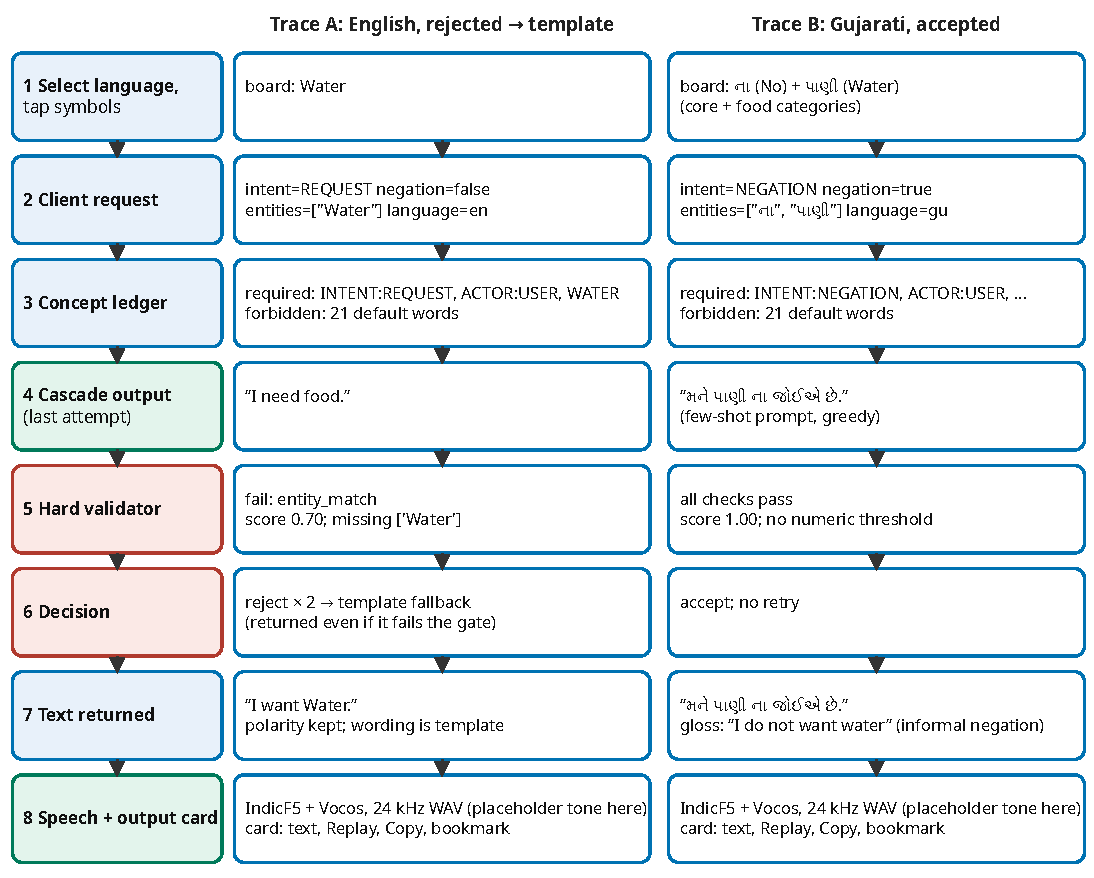
\includegraphics[width=0.86\textwidth]{figures/workflow.pdf}
\caption{Interaction flow for an English request (cascade output rejected twice, template returned) and a Gujarati request (cascade output accepted). English gloss of Trace~B: ``I do not want water'' (informal negation; not native-reviewed).}
\label{fig:workflow}
\end{figure*}

\begin{figure}[t]
\centering
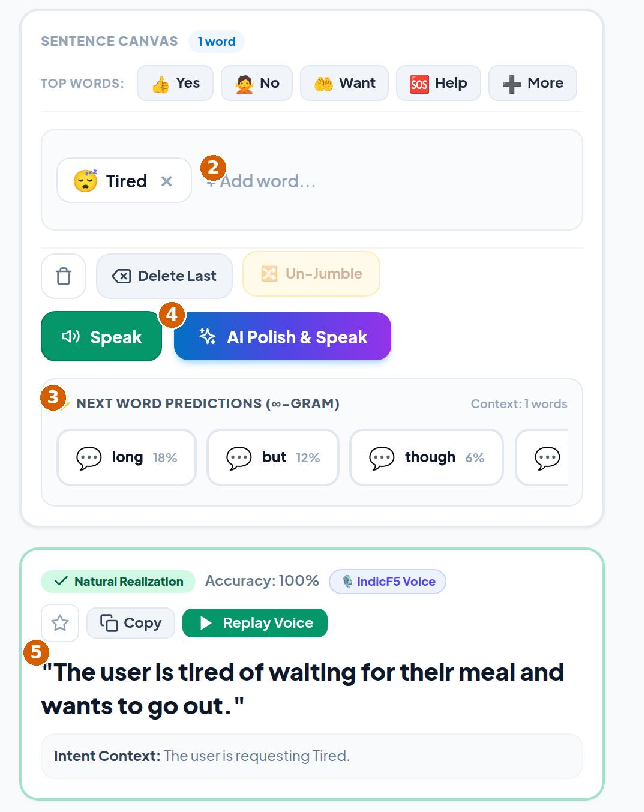
\includegraphics[width=0.72\columnwidth]{figures/ui_failure.pdf}
\caption{English, \emph{Tired}: the client sends \textsc{request}; the gate accepts a fluent sentence that adds unselected content. The card shows ``Accuracy: 100\%''. This screenshot is a different sample from the evaluated one. Callouts as in Figure~\ref{fig:ui}.}
\label{fig:failure}
\end{figure}

\section{Scorer Definitions}
\label{app:scorer}
Retention is the share of required concept instances present (lexicon forms with inflection stems). Polarity is correct when a negator is present exactly if the gold message is negated. The act is correct when a request marker (want, need, \hi{चाहिए}, \gu{જોઈએ}, \hi{हवे}) or, for feelings, a feeling marker without a request marker is present. A concept is \emph{added} if any other board concept or a time, meal or venue word occurs. An output is \emph{off-task} if it is a refusal, a third-person report (``the user\ldots''), empty, longer than 25 tokens, or contains Latin text in an Indic target. Scenarios, lexicon, scorer and raw outputs are in \texttt{eval/}.

\section{Refiner Fine-Tuning and Results}
\label{app:refiner}
The English refiner fine-tunes \texttt{google/flan-t5-small} (revision \texttt{0fc9ddf}, 76,961,152 parameters) to map selected concepts and a user intent to one sentence (Table~\ref{tab:refiner}). Training used fp32 with learning rate $10^{-4}$, weight decay 0.01, batch size 16 with two accumulation steps, 10 epochs (960 updates), source and target limits of 256 and 64 tokens, seed 42, and one NVIDIA TITAN Xp (204\,s, 2.4\,GiB peak); the checkpoint with the lowest validation loss is kept. The fluency arm first adapts for 500 updates on 4,380 denoising pairs. Training, validation and test hold 3,052, 384 and 384 template-generated payloads in 318, 40 and 40 disjoint groups. Because references come from the same template families as the rule path, rule and hybrid scores are exact by construction; the model scores are the informative ones.

\begin{table}[t]
\centering\footnotesize
\setlength{\tabcolsep}{3pt}
\begin{tabular}{@{}lcc@{}}
\toprule
Test (384 payloads) & AAC only & Fluency, then AAC \\
\midrule
Raw selection & \RefARaw{} & \RefFRaw{} \\
Rules & \RefARules{} & \RefFRules{} \\
Fine-tuned model & \RefAModel{} & \RefFModel{} \\
Hybrid (rules + model) & \RefAHybrid{} & \RefFHybrid{} \\
Negation errors (not raw) & 0/172 & 0/172 \\
Model latency, median (ms) & \RefALat{} & \RefFLat{} \\
\bottomrule
\end{tabular}
\caption{Exact match of the refiner, recomputed from the raw predictions of the training kit (it equals the kit's own \texttt{metrics.csv}). The model weights are not in the package; the configuration and tokenizer are.}
\label{tab:refiner}
\end{table}


\end{document}
